\documentclass[12pt]{article}
\usepackage[utf8]{inputenc}

\newenvironment{sol}[1][Solution]{\begin{trivlist}\item[\hskip\labelsep {\bfseries #1:}]}{\end{trivlist}}
\usepackage[margin=1in]{geometry} 
\usepackage{amsmath,amsthm,amssymb}
\usepackage{minted}
\usemintedstyle{vs}
\usepackage{graphicx}
\graphicspath{{./images}}
\usepackage{ amssymb }
\usepackage{times,url}  
\usepackage{hyperref}

\title{CS7381 Project 7: Verilog Code Development – MIPS Data Path Control Unit }
\author{
Name: Bingying Liang \\
ID: 48999397\\  
Distance}
\date{Apr 19 2023}

\begin{document}
\maketitle
For this exercise, you will write a Verilog code program to implement the MIPS ALU Control Unit.    You will test your Control Unit module using the testbench provided in the assignment. 

Recall the following web site links for Verilog help:
\begin{itemize}
    \item \href{http://lyle.smu.edu/~manikas/CAD_tool_info.html} {http://lyle.smu.edu/~manikas/CAD\_tool\_info.html}
    \item \href{https://s2.smu.edu/~manikas/CAD_Tools/Verilog/Xcelium.html}{https://s2.smu.edu/~manikas/CAD\_Tools/Verilog/Xcelium.html}. 
\end{itemize}

\begin{enumerate}
    \item Please download the following Verilog file from the assignment page:
    \begin{enumerate}
        \item \href{https://smu.instructure.com/courses/106177/files/7256739?wrap=1}{S23\_controller\_tb.v} - the testbench for testing your Control Unit
        \item This testbench will have machine code for various MIPS instructions
        \item See the format of the testbench to help you design your control unit
    \end{enumerate}
            \begin{center}
        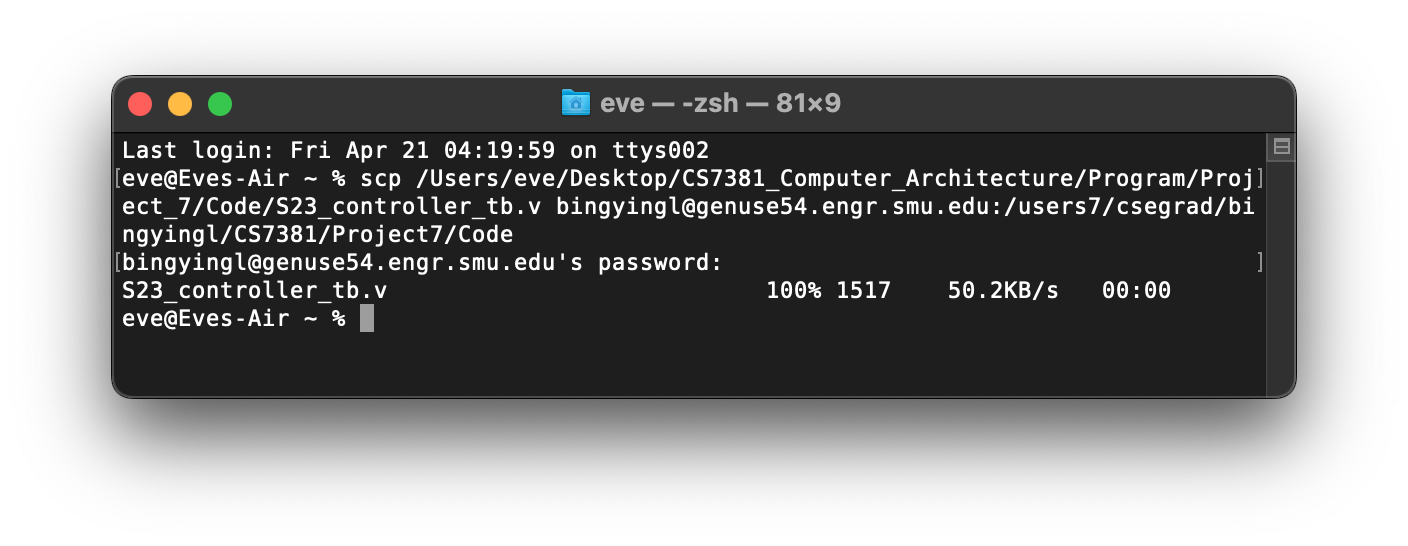
\includegraphics[width=0.9\textwidth]{p1.png}
        \end{center}

        Depending on the testbench we can analyis the right result of these test.
        \begin{center}
            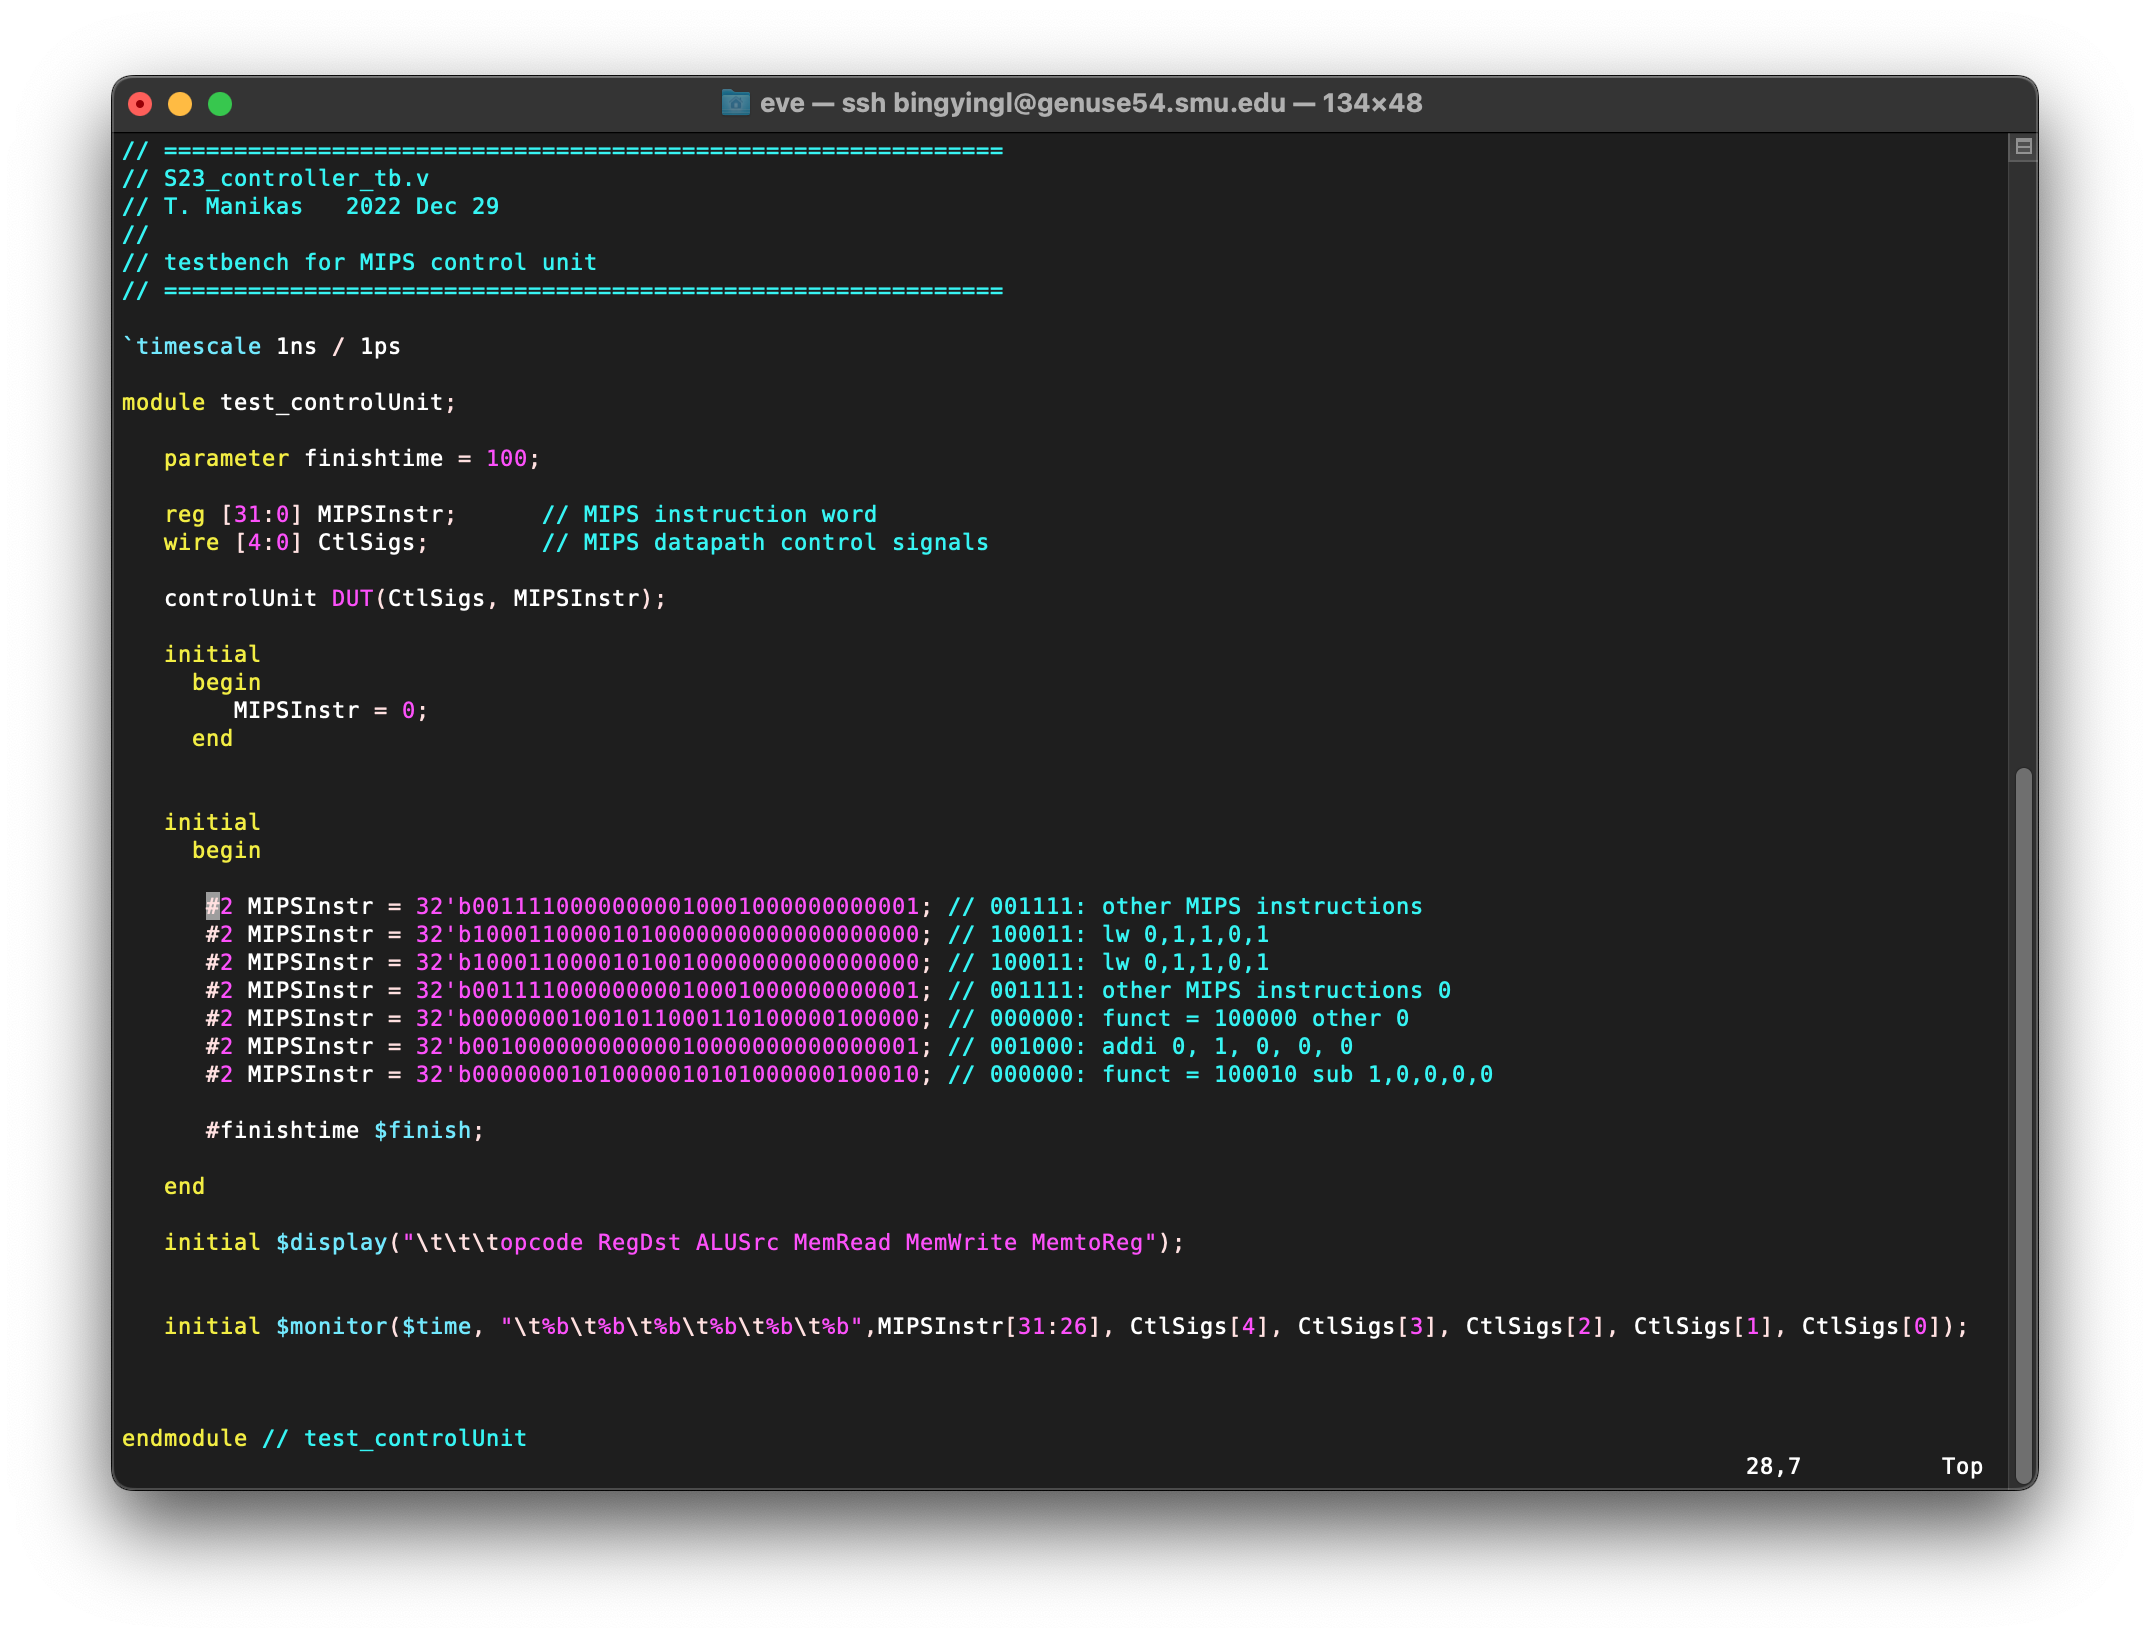
\includegraphics[width=0.9\textwidth]{p2.png}
        \end{center}
    \item For simplicity in design, your control unit will just need to decode the following MIPS instructions: sub, addi, and lw.  
     \begin{minted}[frame=lines,framesep=2mm,baselinestretch=1.2,fontsize=\footnotesize]{c}
sub: R; opcode = 000000; funct = 100010 
addi: I; opcode = 001000;  
lw: I; opcode = 100011; 
\end{minted}
    

    \item For these instructions, your control unit will need to output the correct values for the following control signals:
    \begin{enumerate}
        \item RegDst
        \item ALUSrc
        \item MemRead
        \item MemWrite
        \item MemtoReg
    \end{enumerate}
         \begin{minted}[frame=lines,framesep=2mm,baselinestretch=1.2,fontsize=\footnotesize]{c}
lw: RegDst = 0 ; ALUSrc = 1; MemRead = 1; MemWrite = 0; MemtoReg = 1; 
addi: RegDst = 0; ALUSrc = 1; MemRead = 0; MemWrite = 0; MemtoReg = 0;
sub: RegDst= 1; ALUSrc = 0; MemRead = 0; MemWrite = 0; MemtoReg = 0;
\end{minted}

    \item For other MIPS instructions, set these control signals to 0.
\begin{minted}[frame=lines,framesep=2mm,baselinestretch=1.2,fontsize=\footnotesize]{c}
RegDst = 0 ; ALUSrc = 0; MemRead = 0; MemWrite = 0; MemtoReg = 0;
\end{minted}
    \item Develop the MIPS control unit in Verilog.
    \begin{enumerate}
        \item Save the program as a *.v file – use the first initial of your first name and the first 4 letters of your last name, then the number 3 (to distinguish from your code for previous Verilog projects). For example, my file submission name would be tmani3.v.
                    \begin{center}
        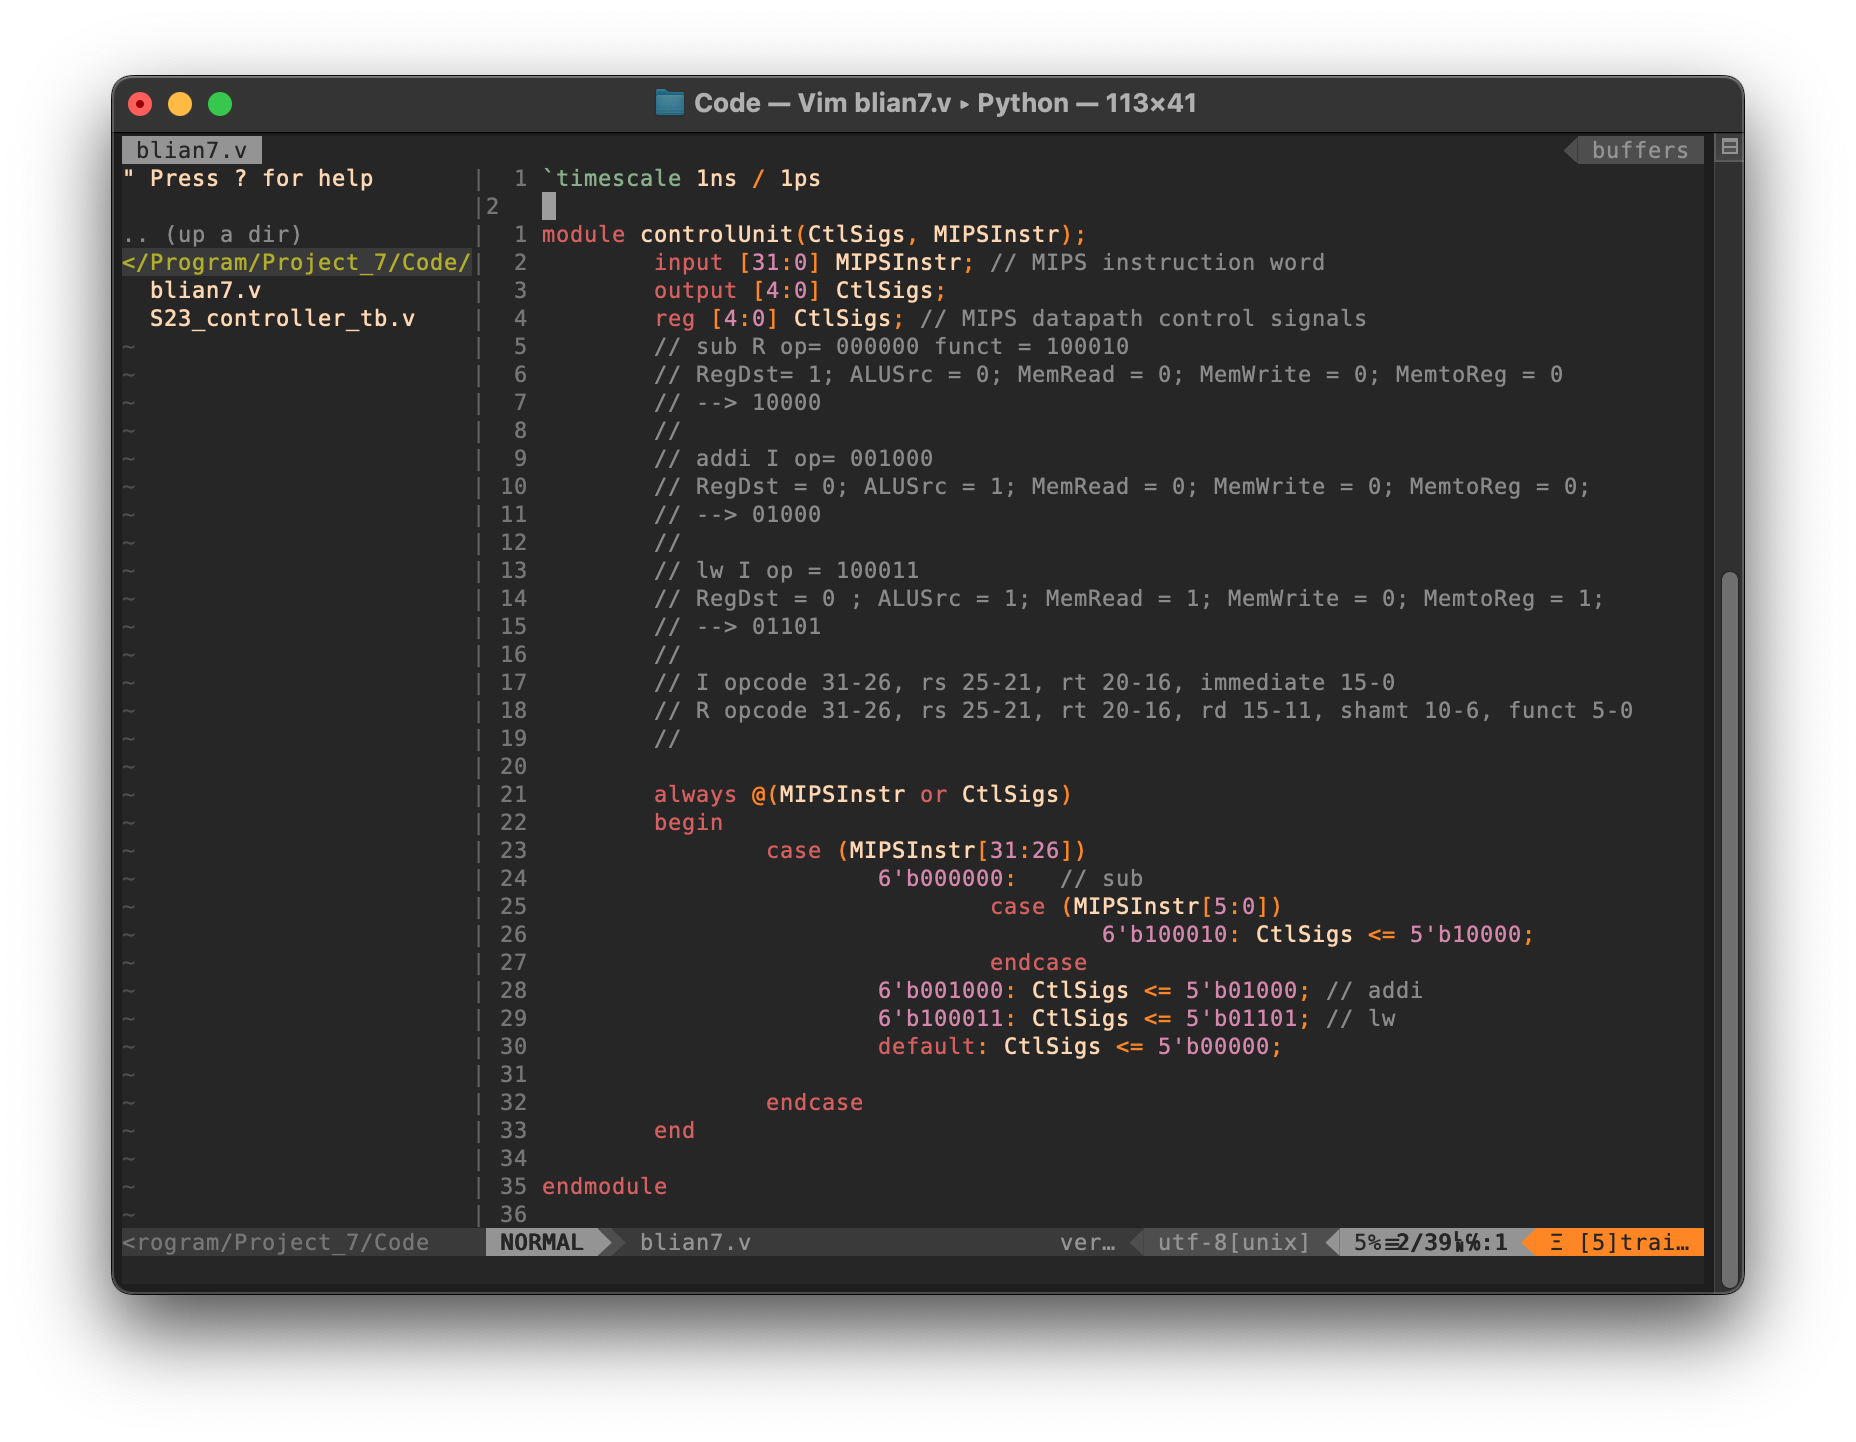
\includegraphics[width=0.9\textwidth]{p3.png}
        \end{center}
        \item Test your Control Unit using the testbench provided in Step 1.
                    \begin{center}
        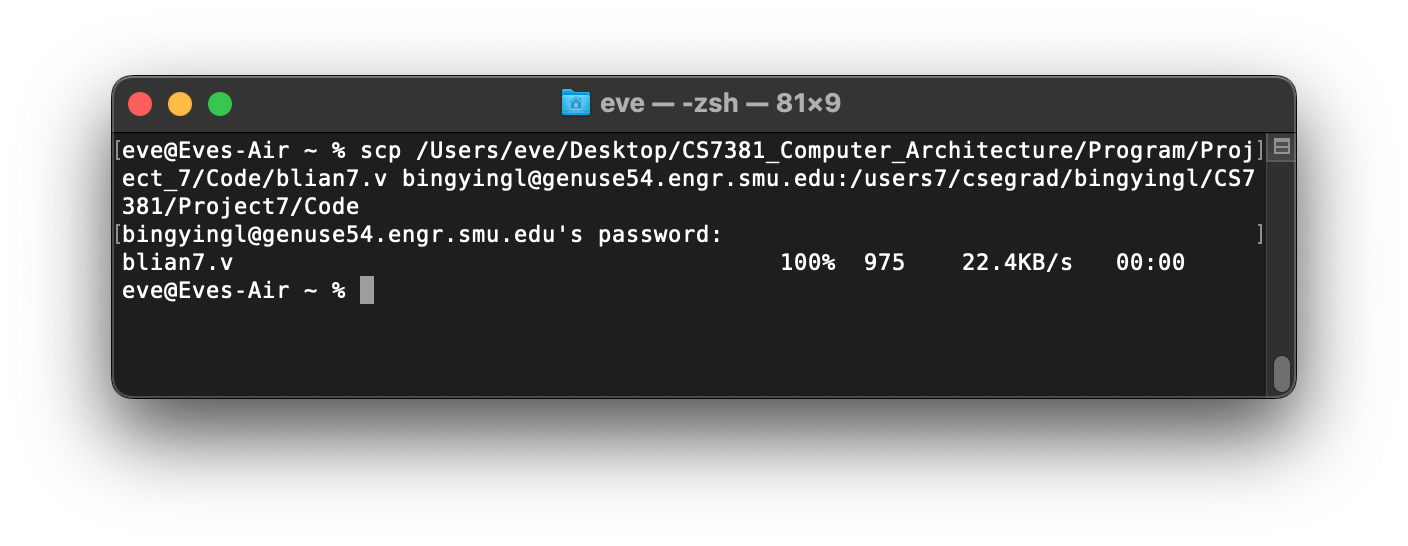
\includegraphics[width=0.9\textwidth]{p4.png}
                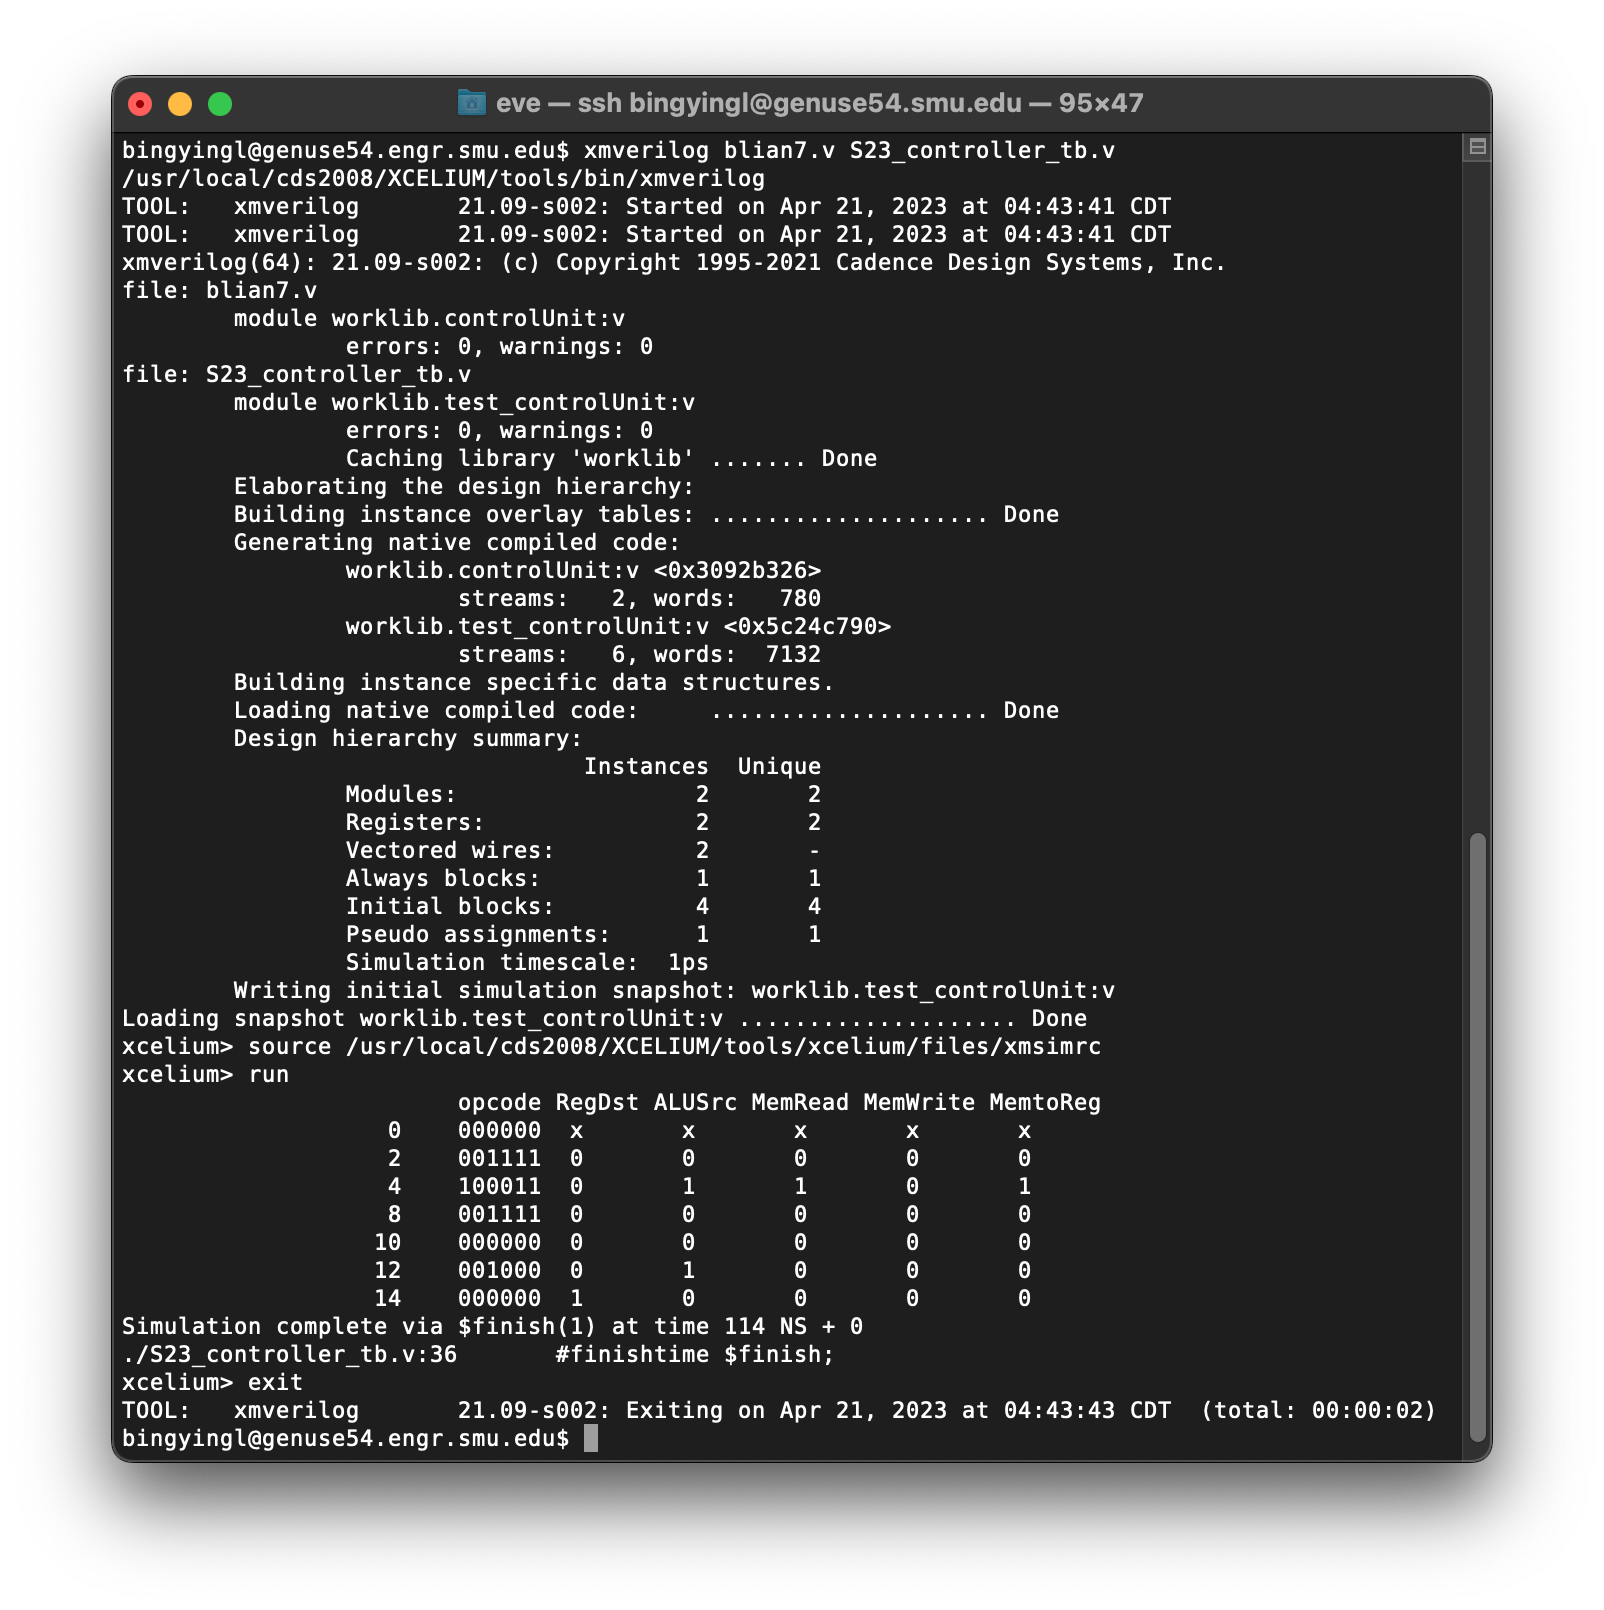
\includegraphics[width=0.9\textwidth]{p5.png}
        \end{center}
                Compare the result with testbench annotation and table they are the same and mapped correctly.
    \end{enumerate}
    \item Please include the following for your homework submission:
    \begin{enumerate}
        \item Your Control Unit Verilog file – submit the actual *.v file so that the grader can run them.
        \begin{center}
        
\includegraphics[width=0.2\textwidth]{p6.png}
        \end{center}
        \item Your testbench results – this can be a copy of the results on a Word document.
        
        I download the result file log from the server and modify the name as blian7.log
                \begin{center}
        
\includegraphics[width=0.9\textwidth]{p7.png}
        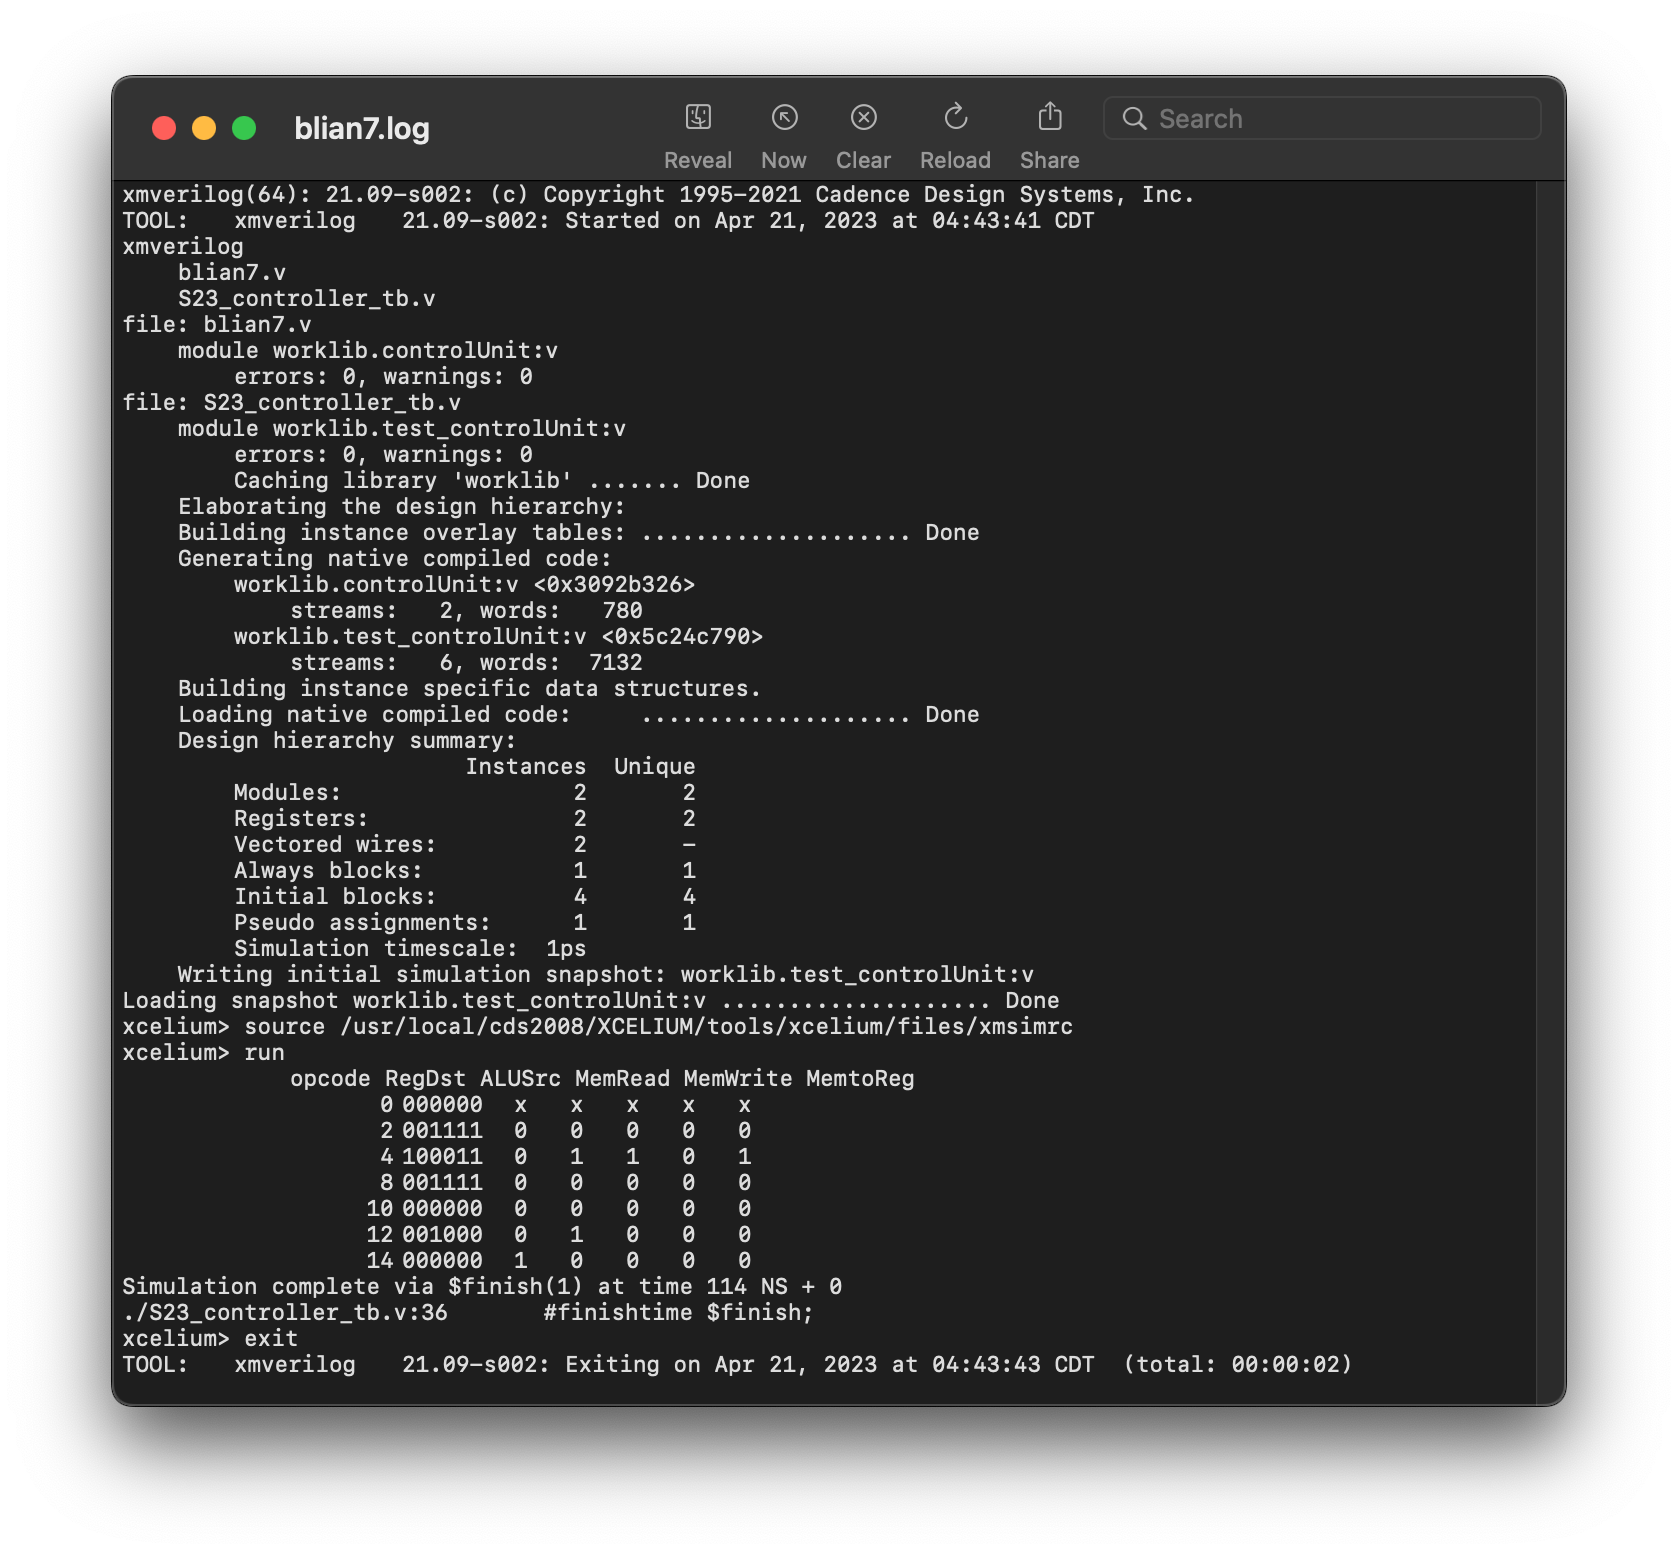
\includegraphics[width=0.9\textwidth]{p8.png}
        \end{center}
        \item PLEASE MAKE SURE THAT YOUR NAME APPEARS ON ALL SUBMITTED ITEMS FOR PROPER CREDIT
    \end{enumerate}
\end{enumerate} 

\end{document}
